\documentclass{article}\usepackage[]{graphicx}\usepackage[]{color}
%% maxwidth is the original width if it is less than linewidth
%% otherwise use linewidth (to make sure the graphics do not exceed the margin)
\makeatletter
\def\maxwidth{ %
  \ifdim\Gin@nat@width>\linewidth
    \linewidth
  \else
    \Gin@nat@width
  \fi
}
\makeatother

\definecolor{fgcolor}{rgb}{0.345, 0.345, 0.345}
\newcommand{\hlnum}[1]{\textcolor[rgb]{0.686,0.059,0.569}{#1}}%
\newcommand{\hlstr}[1]{\textcolor[rgb]{0.192,0.494,0.8}{#1}}%
\newcommand{\hlcom}[1]{\textcolor[rgb]{0.678,0.584,0.686}{\textit{#1}}}%
\newcommand{\hlopt}[1]{\textcolor[rgb]{0,0,0}{#1}}%
\newcommand{\hlstd}[1]{\textcolor[rgb]{0.345,0.345,0.345}{#1}}%
\newcommand{\hlkwa}[1]{\textcolor[rgb]{0.161,0.373,0.58}{\textbf{#1}}}%
\newcommand{\hlkwb}[1]{\textcolor[rgb]{0.69,0.353,0.396}{#1}}%
\newcommand{\hlkwc}[1]{\textcolor[rgb]{0.333,0.667,0.333}{#1}}%
\newcommand{\hlkwd}[1]{\textcolor[rgb]{0.737,0.353,0.396}{\textbf{#1}}}%
\let\hlipl\hlkwb

\usepackage{framed}
\makeatletter
\newenvironment{kframe}{%
 \def\at@end@of@kframe{}%
 \ifinner\ifhmode%
  \def\at@end@of@kframe{\end{minipage}}%
  \begin{minipage}{\columnwidth}%
 \fi\fi%
 \def\FrameCommand##1{\hskip\@totalleftmargin \hskip-\fboxsep
 \colorbox{shadecolor}{##1}\hskip-\fboxsep
     % There is no \\@totalrightmargin, so:
     \hskip-\linewidth \hskip-\@totalleftmargin \hskip\columnwidth}%
 \MakeFramed {\advance\hsize-\width
   \@totalleftmargin\z@ \linewidth\hsize
   \@setminipage}}%
 {\par\unskip\endMakeFramed%
 \at@end@of@kframe}
\makeatother

\definecolor{shadecolor}{rgb}{.97, .97, .97}
\definecolor{messagecolor}{rgb}{0, 0, 0}
\definecolor{warningcolor}{rgb}{1, 0, 1}
\definecolor{errorcolor}{rgb}{1, 0, 0}
\newenvironment{knitrout}{}{} % an empty environment to be redefined in TeX

\usepackage{alltt}%[final]
\setcounter{secnumdepth}{3}
% if you need to pass options to natbib, use, e.g.:
% \PassOptionsToPackage{numbers, compress}{natbib}
% before loading nips_2016
%
% to avoid loading the natbib package, add option nonatbib:
% \usepackage[nonatbib]{nips_2016}

%\usepackage{nips_2016}

% to compile a camera-ready version, add the [final] option, e.g.:
%\usepackage[final]{nips_2016}
\usepackage{amsmath}
\usepackage[utf8]{inputenc} % allow utf-8 input
\usepackage[T1]{fontenc}    % use 8-bit T1 fonts
\usepackage{hyperref}       % hyperlinks
\usepackage{url}            % simple URL typesetting
\usepackage{booktabs}       % professional-quality tables
\usepackage{amsfonts}       % blackboard math symbols
\usepackage{nicefrac}       % compact symbols for 1/2, etc.
\usepackage{microtype}      % microtypography
\usepackage{float}
\usepackage{amssymb}
\usepackage{amsthm}
\usepackage{color,soul}
\usepackage{amsmath}
\usepackage{algorithm}
\usepackage[noend]{algpseudocode}
\usepackage[margin=1.5in]{geometry}
\usepackage[english]{babel}
\usepackage{graphicx}
\usepackage{longtable}

\newtheorem{theorem}{Theorem}[section]
\newtheorem{lemma}[theorem]{Lemma}
\newtheorem{proposition}[theorem]{Proposition}
\newtheorem{corollary}[theorem]{Corollary}
\theoremstyle{definition}
\newtheorem{definition}{Definition}[section]

% Code defs from jss
\newcommand\code{\@codex}
\def\@codex#1{{\normalfont\ttfamily\hyphenchar\font=-1 #1}}
%%\let\code=\texttt
\let\proglang=\textsf
\newcommand{\pkg}[1]{{\fontseries{b}\selectfont #1}}


%\theoremstyle{definition}
%\newtheorem{definition}{Definition}[section]


\makeatletter
\def\BState{\State\hskip-\ALG@thistlm}
\makeatother

\title{Time Series Methods in the R package \pkg{mlr}}

% The \author macro works with any number of authors. There are two
% commands used to separate the names and addresses of multiple
% authors: \And and \AND.
%
% Using \And between authors leaves it to LaTeX to determine where to
% break the lines. Using \AND forces a line break at that point. So,
% if LaTeX puts 3 of 4 authors names on the first line, and the last
% on the second line, try using \AND instead of \And before the third
% author name.

\author{
  Steve Bronder \\
  %Quantitative Methods of the Social Sciences\\
  %Columbia University\\
  %New York City, NY 10027 \\
  \texttt{sab2287@columbia.edu} \\
  %% examples of more authors test etst
   %Department of Computer Science \\
   %Columbia University\\
   %New York City, NY 10027 \\
  %% \AND
  %% Coauthor \\
  %% Affiliation \\
  %% Address \\
  %% \texttt{email} \\
  %% \And
  %% Coauthor \\
  %% Affiliation \\
  %% Address \\
  %% \texttt{email} \\
  %% \And
  %% Coauthor \\
  %% Affiliation \\
  %% Address \\
  %% \texttt{email} \\
}
\IfFileExists{upquote.sty}{\usepackage{upquote}}{}
\begin{document}
% \nipsfinalcopy is no longer used

\maketitle

\begin{abstract}
The \pkg{mlr} package is a unified interface for machine learning tasks such as classification, regression, cluster analysis, and survival analysis. \pkg{mlr} handles the data pipeline of pre-processing, resampling, model selection, model tuning, ensembling, and prediction. This paper details new methods for developing time series  models in \pkg{mlr}. It includes standard and novel tools such as auto-regressive and LambertW transform data generating processes, fixed and growing window cross validation, and forecasting models in the context of univariate and multivariate time series. Examples from forecasting competitions will be given in order to demonstrate the benefits of a unified framework for machine learning and time series.
  \end{abstract}

\section{Introduction}
There has been a rapid developement in time series methods over the last 25 years ~\cite{Hyndman25} whereby time series models have not only become more common, but more complex. The \proglang{R} language ~\cite{Rbase} has a large task view with many packages available for forecasting and time series methods, but the open source nature of R has left users without a standard framework. Many packages have their own sub-culture of style, syntax, and output. The \pkg{mlr} ~\cite{mlr} package, short for Machine Learning in R, works to give a strong syntatic framework for the modeling pipeline. By automating many of the standard tools in machine learning such as preprocessing and cross validation, \pkg{mlr} reduces error from the user during the modeling process. 

While there are some time series methods available in \pkg{caret} ~\cite{caret}, development of forecasting models in \pkg{caret} is difficult due to computational constraints and design choices within the package. The highly modular structure of \pkg{mlr} makes it the best choice for implementing time series methods and models. This paper will show how using \pkg{mlr}'s strong syntatic structure allows for time series packages such as \pkg{forecast} ~\cite{HyndForecast}, \pkg{rugarch} ~\cite{rugarch}, and ~\cite{BigVAR} to use machine learning methedologies such as automated parameter tuning, data preprocessing, model blending, cross validation, performance evaluation, and parallel processing techniques for decreasing model build time.

\section{Forecasting Example with the M4 Competition}
\label{sec:m4data}

Professional forecasters attempt to predict the future of a series based on its past values. Forecasting can be used in a wide range of tasks including forecasting stock prices, ~\cite{GRANGER19923}, weather patterns ~\cite{MurphymeteoForecast}, international conficts ~\cite{Chadefaux01012014}, and earthquakes ~\cite{earthquakeYegu}. In order to evaluate \pkg{mlr}'s forecasting framework we need a large set of possible time series to make sure our methods generalize well.

The Makridakis competitions ~\cite{Makridakis2000451} is a set of forecasting challenges organized by the International Institute of Forecasters and led by Spyros Makridakis to evaluate and compare the accuracy of forecasting methods. The most recent of the competitions, the M4 competition, contains 10,000 time series on a yearly, quarterly, monthly, and daily frequency in areas such as finance, macroeconomics, climate, microeconomics, and industry. To show examples of how \pkg{mlr}'s forecasting features works we will look at a particular climate series. The data is daily with the training subset starting on September 6th, 2007 and ending on September 5th, 2009 while the testing subset is from September 6th, 2009 to October 10th, 2009 for a total of 640 training periods and 35 test periods to forecast.


\begin{knitrout}
\definecolor{shadecolor}{rgb}{0.969, 0.969, 0.969}\color{fgcolor}

{\centering 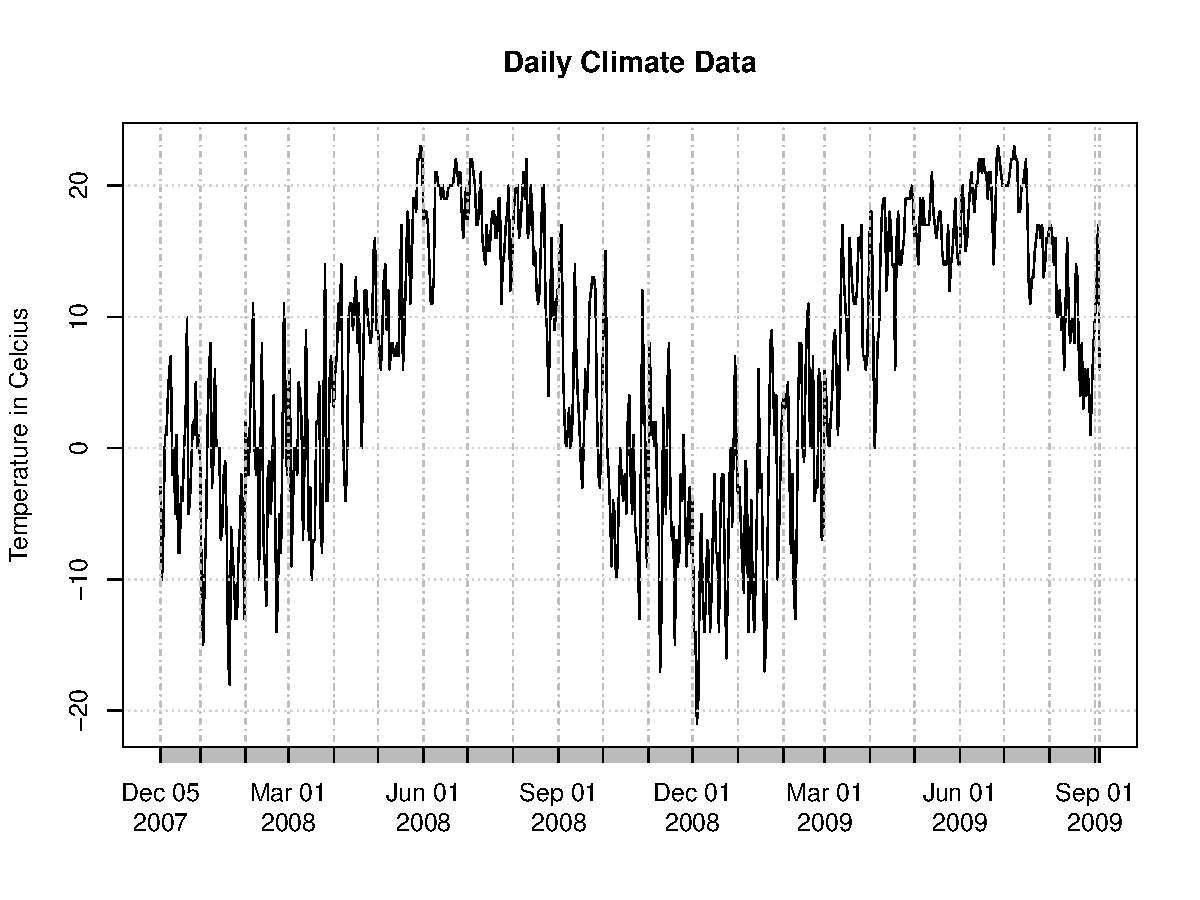
\includegraphics[width=\maxwidth]{figure/get_dat_weather-1} 

}



\end{knitrout}

This series was chosen for its obvious seasonality and time features. Our data set should be large enough that the tuning method can take multiple windows of the data. Some series in M4 only contain 12 observations, which is not enough data to accurately train a model. We can see figure one is what most people imagine when they think of a time series. There is a clear seasonal time trend with individual points moving about the seasonal periods. The data can be found in the package \pkg{M4comp} ~\cite{m4comp} under sets \code{M4[28]} and \code{M4[29]}. 

For multivariate forecasting, we will use the EUStockMarkets data set from the \pkg{datasetes} ~\cite{datasets}. It contains a set of DAX, SMI, CAC, and FTSE European stock indices from July 1st, 1991 to August 24th, 1998 totaling 1828 training observations and 32 test observations.

\begin{knitrout}
\definecolor{shadecolor}{rgb}{0.969, 0.969, 0.969}\color{fgcolor}

{\centering 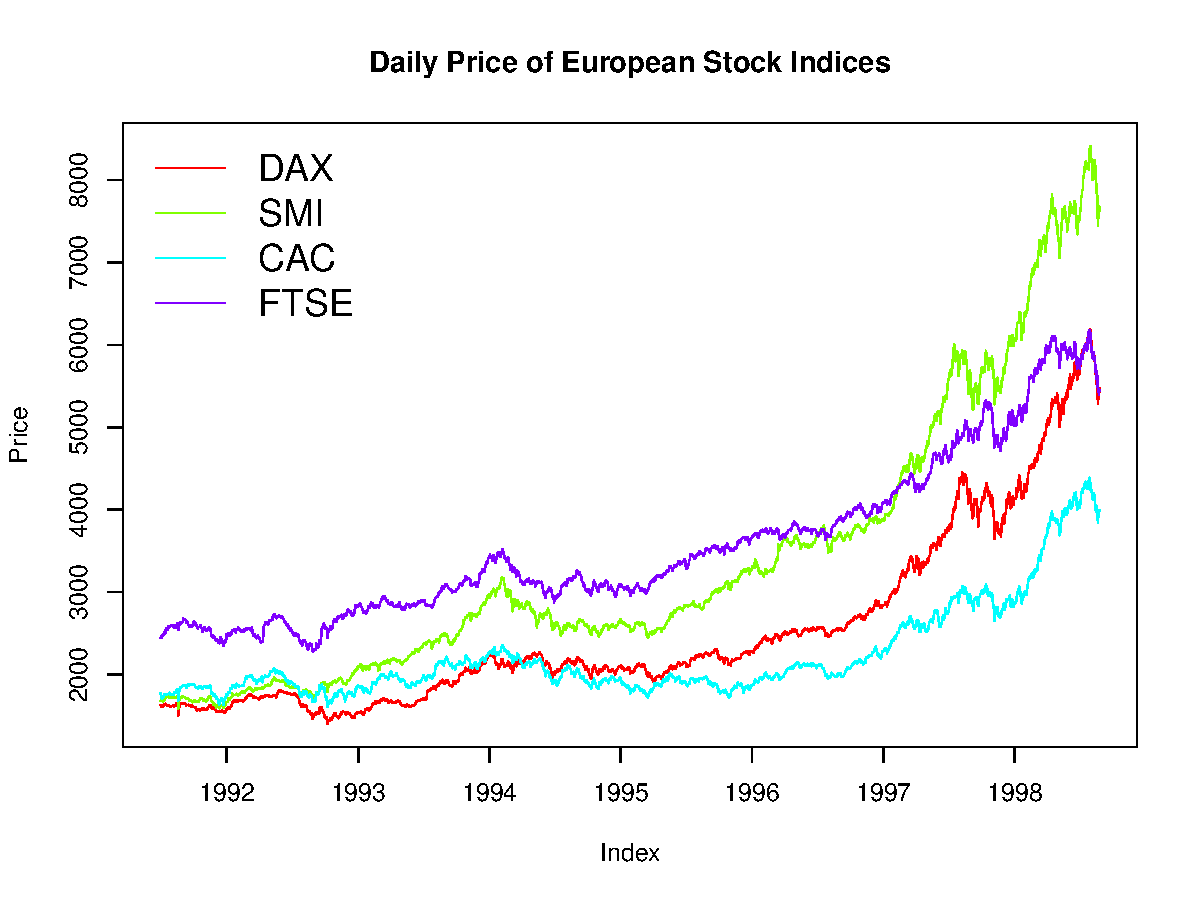
\includegraphics[width=\maxwidth]{figure/get_dat_stocks-1} 

}



\end{knitrout}

Note that each stock index tends to follow a similar, but diverging, trend. This will be important to note when we perform windowing cross validation as it will let us see how well the models adapt to what appears to be nonstationary data.

\section{Univariate and Multivariate Forecasting Tasks}
\label{sec:task}

\pkg{mlr} uses the S3 object system to clearly define a predictive modeling task. Tasks contain the data and other relevant information such as the task id and which variable you are targeting for supervised learning problems. Forecasting tasks are handled in \pkg{mlr} by the function \code{makeForecastRegrTask()}. The forecasting task inherets most of it's arguments from \code{makeRegrTask}, but has two noticable differences in arguments.

\begin{itemize}
\item[data:] Instead of a data frame, an xts object from \pkg{xts} ~\cite{xts} containing the time series.
\item[frequency:] An integer with the number of periods your time series contains. For example, daily data with a weekly periodicity has a frequency of 7, daily data with a yearly periodicity has a frequency of 365, and weekly data with a yearly frequency has a periodicity of 52.
\end{itemize}

\begin{knitrout}
\definecolor{shadecolor}{rgb}{0.969, 0.969, 0.969}\color{fgcolor}\begin{kframe}
\begin{alltt}
\hlkwd{library}\hlstd{(mlr)}
\hlstd{climate.task} \hlkwb{=} \hlkwd{makeForecastRegrTask}\hlstd{(}\hlkwc{id} \hlstd{=} \hlstr{"M4 Climate Data"}\hlstd{,}
                                 \hlkwc{data} \hlstd{= m4.train,}
                                 \hlkwc{target} \hlstd{=} \hlstr{"target_var"}\hlstd{,}
                                 \hlkwc{frequency} \hlstd{=} \hlnum{183L}\hlstd{)}
\hlstd{climate.task}
\end{alltt}
\begin{verbatim}
## Task: M4 Climate Data
## Type: fcregr
## Target: target_var
## Observations: 640
## Dates:
##  Start: 2007-12-05 
##  End:   2009-09-04
## Frequency: 183
## Features:
## numerics  factors  ordered 
##        0        0        0 
## Missings: FALSE
## Has weights: FALSE
## Has blocking: FALSE
\end{verbatim}
\end{kframe}
\end{knitrout}

Like a regression task, this records the type of the learning problem and basic information about the data set such as the start and end dates, frequency, and whether we have missing values. Note that there are zero features in our task because we only have a target variable, which the model itself will use to build features.

One common problem with forecasting is that it is difficult to use additional explanatory variables or forecast multiple targets that are dependent on one another. If we are at time $t$ and want to forecast 10 periods in the future, we need to know the values of the explanatory variables at time $t+10$, which is often not possible. A new set of models ~\cite{BigVAR} which treats explanatory variables endogenously instead of exogenously allows us to forecast not only our target, but addititional explanatory variables. This is done by treating all the variables as targets, making them endogeneous to the model. To use these models, we create a multivariate forecasting task. The function \code{makeMultiForecastRegrTask()} has the same arguments as \code{makeForecastRegrTask()} with one exception. The \code{target} argument can contain either a single target variable, multiple target variables, or \code{All} which treats all variables endogeneously.

\begin{knitrout}
\definecolor{shadecolor}{rgb}{0.969, 0.969, 0.969}\color{fgcolor}\begin{kframe}
\begin{alltt}
\hlstd{mfcregr.univar.task} \hlkwb{=} \hlkwd{makeMultiForecastRegrTask}\hlstd{(}\hlkwc{id} \hlstd{=} \hlstr{"bigvar"}\hlstd{,}
                                                \hlkwc{data} \hlstd{= EuStockMarkets,}
                                                \hlkwc{target} \hlstd{=} \hlstr{"FTSE"}\hlstd{,}
                                                \hlkwc{frequency} \hlstd{=} \hlnum{365L}\hlstd{)}
\end{alltt}


{\ttfamily\noindent\bfseries\color{errorcolor}{\#\# Error in eval(expr, envir, enclos): could not find function "{}makeMultiForecastRegrTask"{}}}\begin{alltt}
\hlstd{mfcregr.univar.task}
\end{alltt}


{\ttfamily\noindent\bfseries\color{errorcolor}{\#\# Error in eval(expr, envir, enclos): object 'mfcregr.univar.task' not found}}\end{kframe}
\end{knitrout}

Like \code{makeForecastRegrTask()}, \code{mfcregr.univar.task} we get the standard output, but notice now that there are three three features. Alternatively, \code{mfcregr.all.task} contains multiple target values with no features. The difference between each of these multivariate tasks is that \code{mfcregr.univar.task} will act similar to \code{makeForecastRegrTask()}, giving the output, predictions, and even using the measures for univariate forecasting tasks. Both of these tasks will still forecast all of the underlying series, which allows us take exogeneous models and treat them endogeneously for multi-step forecasts.

\begin{knitrout}
\definecolor{shadecolor}{rgb}{0.969, 0.969, 0.969}\color{fgcolor}\begin{kframe}
\begin{alltt}
\hlstd{mfcregr.all.task} \hlkwb{=} \hlkwd{makeMultiForecastRegrTask}\hlstd{(}\hlkwc{id} \hlstd{=} \hlstr{"bigvar"}\hlstd{,}
                                             \hlkwc{data} \hlstd{= eu.train,}
                                             \hlkwc{target} \hlstd{=} \hlstr{"all"}\hlstd{,}
                                             \hlkwc{frequency} \hlstd{=} \hlnum{365L}\hlstd{)}
\end{alltt}


{\ttfamily\noindent\bfseries\color{errorcolor}{\#\# Error in eval(expr, envir, enclos): could not find function "{}makeMultiForecastRegrTask"{}}}\begin{alltt}
\hlstd{mfcregr.all.task}
\end{alltt}


{\ttfamily\noindent\bfseries\color{errorcolor}{\#\# Error in eval(expr, envir, enclos): object 'mfcregr.all.task' not found}}\end{kframe}
\end{knitrout}

\section{Building and Tuning a forecast learner}

\subsection{Univariate Forecasting}

The \code{makeLearner()} function provides a structured model building framework to the several forecasting models currently implimented in \pkg{mlr}. As an example, we will build the Trigonometric exponential smoothing state space model with Box-Cox transformation, ARMA errors, Trend and Seasonal Components (TBATS)~\cite{tbats}. To creae the original BATS model we let $y_t^{\omega}$ be a box cox transformed observation with parameter $\omega$. Then let $m_T$ be the seasonal periods, $l_t$ be the local level in the period, $b$ the long term trend with $b_t$ being the short term trend, $s_t^i$ being the $i$th seasonal component, $d_t$ being an ARIMA($p,q$) model with gaussian white noise process $\epsilon_t$. Smoothing parameters are given by $\alpha$, $\beta$, and $\gamma$ and $\phi$ is the damping constant of the trend.

\begin{align}
y_t^{\omega} &= \begin{cases} 
    \frac{y_t^{\omega} - 1}{\omega}, \omega \ne 0\\
    log(y_t), \omega = 0
    \end{cases}\\
y_t^{\omega} &= l_{t-1} + \phi b_{t-1} + \sum_{i=1}^T s_{t-m_i}^i + d_t\\
l_t &= l_{t-1} + \phi b_{t-1} + \alpha d_t \\
b_t &= (1-\phi)b + \phi b_{t-1} + \beta d_t \\
s_t^i &= s_{t-m_i}^i + \gamma_i d_t \\
d_t &= \sum_{i=1}^p \psi_i d_{t-i} + \sum_{i=1}^q \theta_i \epsilon_{t-i} + \epsilon
\end{align}

The trigonometric part of the model comes from the representation of the seasonal components based on fourier series ~\cite{fourierTrans}. Let the stochastic level of the $i$th seasonal component be $s_{j,t}^{(i)}$ and the stochastic growth in the level of the $i$th seasonal component that is needed to describe the change in the seasonal component over time by $s_{j,t}^{*(i)}$. 

\begin{align}
s_t^{(i)} &= \sum_{j=1}^{k_i} s_{j,t}^{(i)}\\
s_{j,t}^{(i)} &= s_{j,t-1}^{(i)} \cos\lambda_j^{(i)} + s_{j,t-1}^{(i)}\sin\lambda_j^{(i)} + \gamma_1^{(i)}d_t\\
s_{j,t}^{*(i)} &= -s_{j,t-1} \sin\lambda_j^{(i)} + s_{j,t-1}^{*(i)}\cos\lambda_j^{(i)} + \gamma_2^{(i)}d_t
\end{align}

The smoothing parameters are defined by $\gamma_1^{(i)}$ and $\gamma_2^{(i)}$ with $\lambda_j^{(i)} = 2\pi j/m_i$ being a trigonometric smoothing parameter associated with the seasonal periods. The parameter $k_i$ is number of harmonics necessary in the $i$th seasonal component. It's possible to show a simpler deterministic representation of the seasonal components by setting the smoothing parameters to zero. The TBATS model is created by replacing the seasonal component $s_t^{(i)}$ in equation 5 with the trigonometric seasonal equations as well as replacing the measure equation in 2 with 

\begin{equation}
y_t^{\omega} = l_{t-1} + \phi b_{t-1} + \sum_{i=1}^T s_{t-1}^{(i)} + d_t
\end{equation}

TBATS is one of the most well known forecasting models and is available in mlr along with models such as BATS, ARIMA, ETS, several GARCH variants, and autoregressive neural networks. In addition, preprocessing features have been added to allow arbitrary supervised machine learning models to be used in the context of forecasting. To impliment the TBATS model we use  \code{makeLearner()}, supplying the class of learner, order, the number of steps to forecast, and any additional arguments to be passed to \code{tbats} for \pkg{forecast}. 

\begin{knitrout}
\definecolor{shadecolor}{rgb}{0.969, 0.969, 0.969}\color{fgcolor}\begin{kframe}
\begin{alltt}
\hlstd{tbats.mod} \hlkwb{=}\hlkwd{makeLearner}\hlstd{(}\hlstr{"fcregr.tbats"}\hlstd{,} \hlkwc{use.box.cox} \hlstd{=} \hlnum{TRUE}\hlstd{,}
                      \hlkwc{use.trend} \hlstd{=} \hlnum{TRUE}\hlstd{,}
                      \hlkwc{seasonal.periods} \hlstd{=} \hlnum{TRUE}\hlstd{,} \hlkwc{max.p} \hlstd{=} \hlnum{60}\hlstd{,} \hlkwc{max.q} \hlstd{=} \hlnum{60}\hlstd{,}
                      \hlkwc{stationary} \hlstd{=} \hlnum{FALSE}\hlstd{,} \hlkwc{use.arma.errors} \hlstd{=} \hlnum{TRUE}\hlstd{,}
                      \hlkwc{h} \hlstd{=} \hlnum{35}\hlstd{,} \hlkwc{predict.type} \hlstd{=} \hlstr{"response"}\hlstd{)}
\end{alltt}
\end{kframe}
\end{knitrout}

We can also supply a predict type for forecasting models to either receive point estimates (\code{response}) or point estimates with quantiles of confidence intervals (\code{quantile}). To train the model we simply call train, supplying the forecasting model and task. After training the model it's simple to get our forecasts by calling \code{predict()} with the test data, returning an object containing meta information for the forecasts along with the prediction and test data in columns \code{truth} and \code{response}, respectively.

\begin{knitrout}
\definecolor{shadecolor}{rgb}{0.969, 0.969, 0.969}\color{fgcolor}\begin{kframe}
\begin{alltt}
\hlstd{train.tbats}\hlkwb{=} \hlkwd{train}\hlstd{(}\hlkwc{learner} \hlstd{= tbats.mod,} \hlkwc{task} \hlstd{= climate.task )}
\hlstd{train.tbats}
\end{alltt}
\begin{verbatim}
## Model for learner.id=fcregr.tbats; learner.class=fcregr.tbats
## Trained on: task.id = M4 Climate Data; obs = 640; features = 0
## Hyperparameters: use.box.cox=TRUE,use.trend=TRUE,seasonal.periods=TRUE,max.p=60,max.q=60,stationary=FALSE,use.arma.errors=TRUE,h=35
\end{verbatim}
\begin{alltt}
\hlstd{predict.tbats} \hlkwb{=} \hlkwd{predict}\hlstd{(train.tbats,} \hlkwc{newdata} \hlstd{= m4.test)}
\end{alltt}
\end{kframe}
\end{knitrout}

To measure the performane of TBATS we call \code{performance()} with the Mean Absolute Scaled Error (MASE) ~\cite{Hyndman2006} measure.

\begin{knitrout}
\definecolor{shadecolor}{rgb}{0.969, 0.969, 0.969}\color{fgcolor}\begin{kframe}
\begin{alltt}
\hlkwd{performance}\hlstd{(predict.tbats, mase,} \hlkwc{task} \hlstd{= climate.task)}
\end{alltt}
\begin{verbatim}
##      mase 
## 0.0676601
\end{verbatim}
\end{kframe}
\end{knitrout}

MASE has favorable properties for calculating forecast errors relative to measures such as mean root mean squared error or median relative absolute error. Arguably one of the most important features, it's very interpretable. Let $y_t$ and $\tilde{y_t}$ be the target variable and prediction at time $t$ until the final time $T$ with $\epsilon_t = y_t - \tilde{y_t}$ being the forecast error. 

\begin{equation}
\text{MASE} = \frac{\sum_{t=1}^T |\epsilon_t|}{\frac{T}{T-1} \sum_{t=2}^T |y_t - y_{t-1}|}
\end{equation}

Where the denominator is the one step ahead naive forecast from the training data. When the numerator is equal to the denominator the model performed as good as a simple naive forecast method. Scores greater than one mean you are performing worse and scores less than one mean you are performing better.

The scale invariance of MASE means that it is independent of the scale of the data which allows models to be compared across data sets. The scale invariance of MASE has made it a favorite for comparing the accuracy of forecasts methods ~\cite{noteMase}. While scaling in measures such as the Mean Absolute Percentage Error can cause poor behavior as the target variable goes to zero, MASE does not become skewed when the target variable goes to zero. This allows MASE to be use in situations in which zeros occur frequently or zero is not meaningful such as predicting temperature. 

\begin{knitrout}
\definecolor{shadecolor}{rgb}{0.969, 0.969, 0.969}\color{fgcolor}
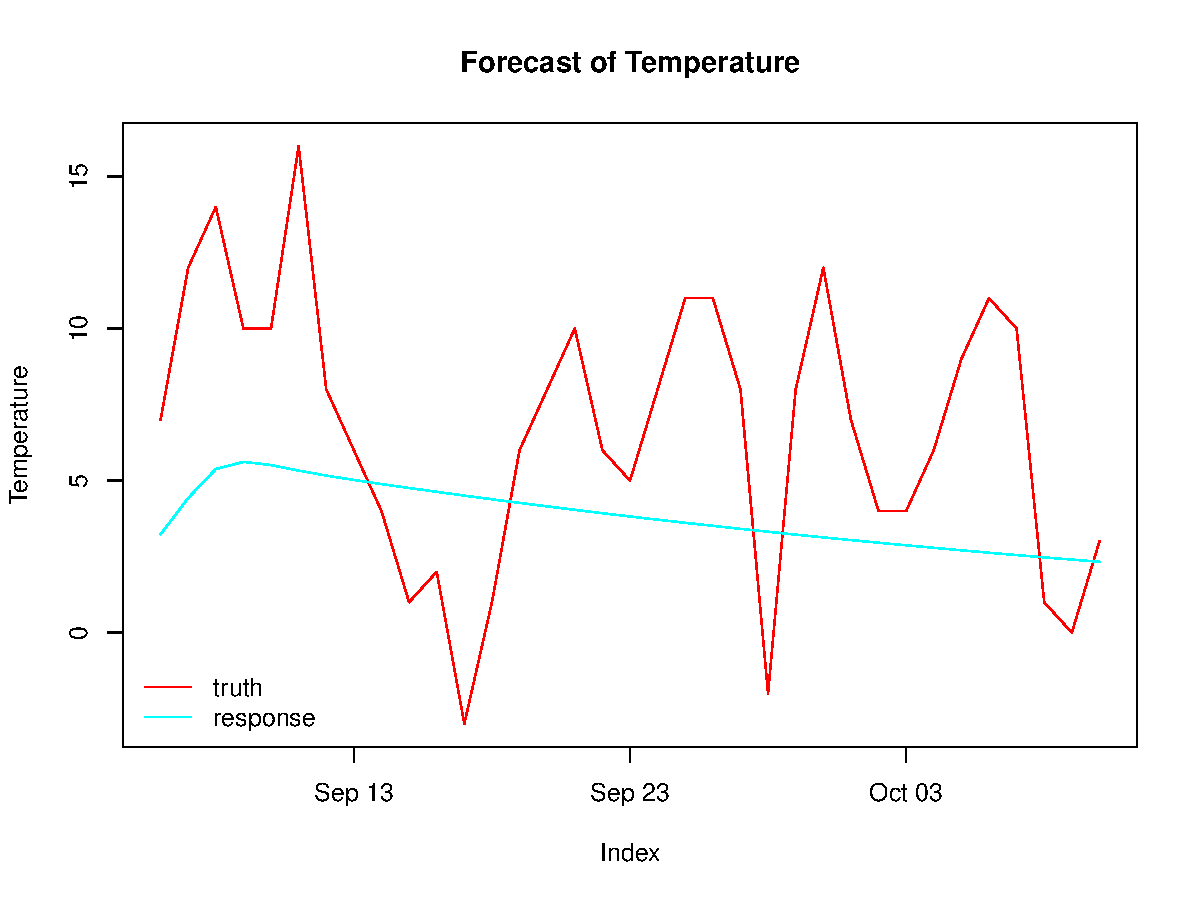
\includegraphics[width=\maxwidth]{figure/plotbatsTrain-1} 

\end{knitrout}

Need to talk about results

Because the forecasts are only for the next 35 periods it's useful to be able to update the model continuously without retraining the model each time we want new forecasts. Univariate forecasting models in \pkg{mlr} can be updated using \code{updateModel()}. 

\begin{knitrout}
\definecolor{shadecolor}{rgb}{0.969, 0.969, 0.969}\color{fgcolor}\begin{kframe}
\begin{alltt}
\hlstd{update.tbats} \hlkwb{=} \hlkwd{updateModel}\hlstd{(train.tbats, climate.task,} \hlkwc{newdata} \hlstd{= m4.test)}
\hlstd{update.tbats}
\end{alltt}
\begin{verbatim}
## Model for learner.id=fcregr.tbats; learner.class=fcregr.tbats
## Trained on: task.id = M4 Climate Data; obs = 35; features = 0
## Hyperparameters: use.box.cox=TRUE,use.trend=TRUE,seasonal.periods=TRUE,max.p=60,max.q=60,stationary=FALSE,use.arma.errors=TRUE,h=35
\end{verbatim}
\begin{alltt}
\hlkwd{predict}\hlstd{(update.tbats,} \hlkwc{task} \hlstd{= climate.task)}
\end{alltt}
\begin{verbatim}
## Prediction: 35 observations
## predict.type: response
## threshold: 
## time: 0.00
##                     response
## 2009-09-04 23:59:54 6.319959
## 2009-09-05 23:59:48 7.875401
## 2009-09-06 23:59:43 8.209328
## 2009-09-07 23:59:37 8.157638
## 2009-09-08 23:59:31 8.083591
## 2009-09-09 23:59:26 8.055280
## ... (35 rows, 1 cols)
\end{verbatim}
\end{kframe}
\end{knitrout}

\subsection{Multivariate Forecasting}

Need to write things for this

\begin{knitrout}
\definecolor{shadecolor}{rgb}{0.969, 0.969, 0.969}\color{fgcolor}\begin{kframe}
\begin{alltt}
\hlstd{bigvar.mod} \hlkwb{=} \hlkwd{makeLearner}\hlstd{(}\hlstr{"mfcregr.BigVAR"}\hlstd{,}\hlkwc{p} \hlstd{=} \hlnum{5}\hlstd{,} \hlkwc{struct} \hlstd{=} \hlstr{"SparseLag"}\hlstd{,}
                         \hlkwc{gran} \hlstd{=} \hlkwd{c}\hlstd{(}\hlnum{50}\hlstd{,} \hlnum{60}\hlstd{),}\hlkwc{h} \hlstd{=} \hlnum{35}\hlstd{,} \hlkwc{n.ahead} \hlstd{=} \hlnum{35}\hlstd{)}
\end{alltt}
\end{kframe}
\end{knitrout}

\begin{knitrout}
\definecolor{shadecolor}{rgb}{0.969, 0.969, 0.969}\color{fgcolor}\begin{kframe}
\begin{alltt}
\hlstd{train.bigvar} \hlkwb{=} \hlkwd{train}\hlstd{(}\hlkwc{learner} \hlstd{= bigvar.mod,} \hlkwc{task} \hlstd{= mfcregr.all.task )}
\hlstd{train.bigvar}
\end{alltt}
\end{kframe}
\end{knitrout}

\begin{knitrout}
\definecolor{shadecolor}{rgb}{0.969, 0.969, 0.969}\color{fgcolor}\begin{kframe}
\begin{verbatim}
## Model for learner.id=mfcregr.BigVAR; learner.class=mfcregr.BigVAR
## Trained on: task.id = bigvar; obs = 1828; features = 0
## Hyperparameters: p=5,struct=SparseLag,gran=50,60,h=35,n.ahead=35
\end{verbatim}
\end{kframe}
\end{knitrout}

\begin{knitrout}
\definecolor{shadecolor}{rgb}{0.969, 0.969, 0.969}\color{fgcolor}\begin{kframe}
\begin{alltt}
\hlstd{predict.bigvar} \hlkwb{=} \hlkwd{predict}\hlstd{(train.bigvar,} \hlkwc{newdata} \hlstd{= eu.test)}
\hlkwd{performance}\hlstd{(predict.bigvar, multivar.mase,} \hlkwc{task} \hlstd{= mfcregr.all.task)}
\end{alltt}
\begin{verbatim}
## multivar.mase 
##     0.2340861
\end{verbatim}
\end{kframe}
\end{knitrout}

\begin{knitrout}
\definecolor{shadecolor}{rgb}{0.969, 0.969, 0.969}\color{fgcolor}
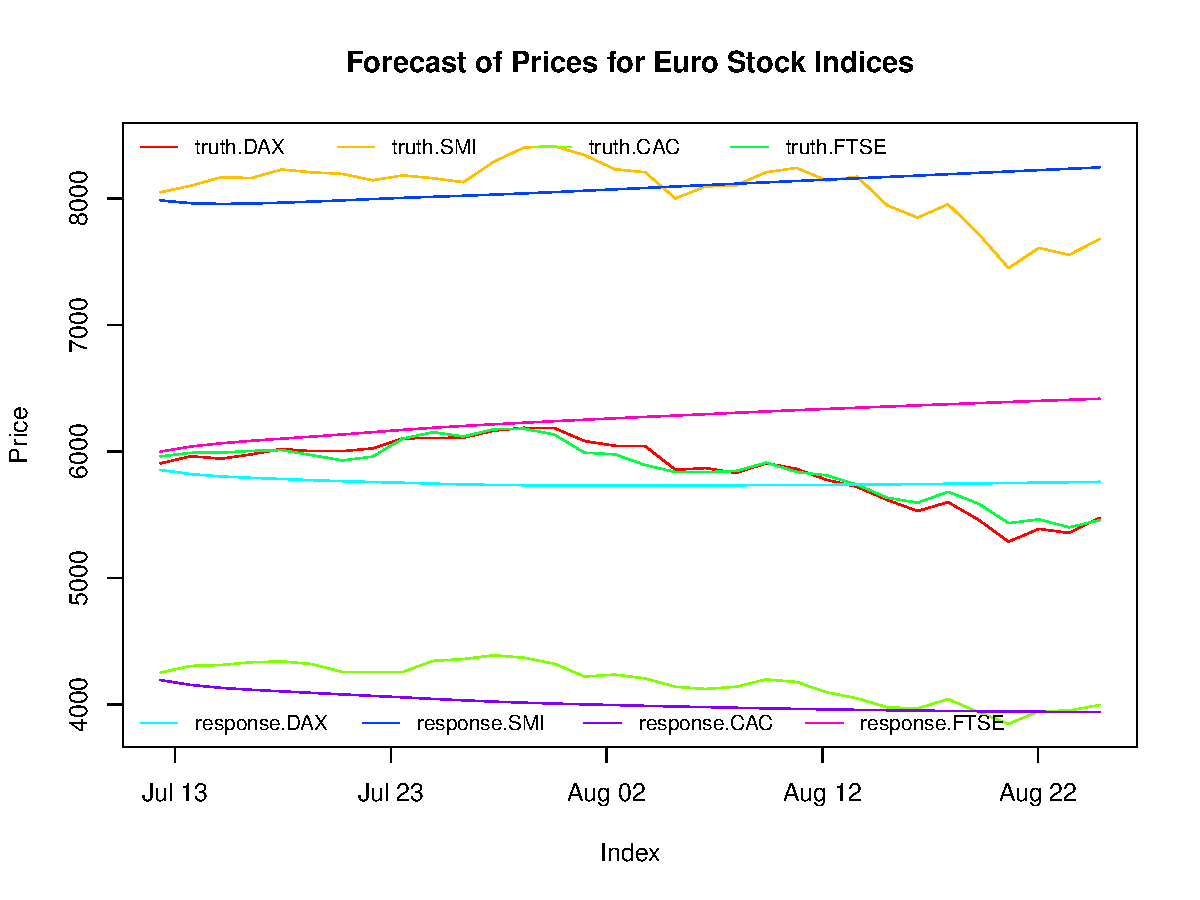
\includegraphics[width=\maxwidth]{figure/bigVarplot-1} 

\end{knitrout}

\section{Resampling with Time}

While TBATS is one of the most well known time series models, the order selection process or the ARIMA errors and whether to include trend, damped trend, or seasonal periods can be a subjective process that makes finding the best model difficult for users. One of the first proposals for automated forecasting methods comes from ~\cite{hannanOrder} for automatic order selection of ARIMA models. Innovations are obtained by fitting high order autoregressive models to the data and then computing the likelihood of potential models through a series of standard regresssions. Proprietary algorithms from software such as \proglang{Forecast Pro} ~\cite{forecastpro} and \proglang{Autobox} ~\cite{reillyautobox} are well known and have performed to high standards in competitions such as the M3 forecasting competition ~\cite{Makridakis2000451}. One of the most well known R packages for automated forecast is \pkg{forecast} ~\cite{HyndForecast} which contains several methods for automated forecasting including exponential smoothing based methods and step-wise algorithms for forecasting with ARIMA models.

Forecasting in \pkg{mlr} takes a machine learning approach, creating a parameter set for a given model and using an optimization method to search over the parameter space. To do this, we will use a windowing resampling scheme to train over the possible models. Resampling schemes such as cross-validation, bootstrapping, etc. are common in machine learning for dealing with the bias-variance tradeoff ~\cite{Friedman1997} ~\cite{rodriguezkfold}. When their is a time component to the data, windowing schemes are useful in allowing a valid resampling scheme while still maintaining the time properties of the series. Figure one gives an example of fixed and growing windows. Given a horizon and initial starting point the window slides forward one step each time while either shifting in the fixed case or enlarging by one in the growing case. Growing and fixed window resampling such as from ~\cite{hyndman2014forecasting} are now available in the \code{resampling()} function of \pkg{mlr}. 

\begin{figure}[ht]
\caption{Resampling with a window scheme as exampled by caret ~\cite{windowingcaret}. The top graphs are fixed window cross validation while the bottom graphs are growing window cross validation. }
  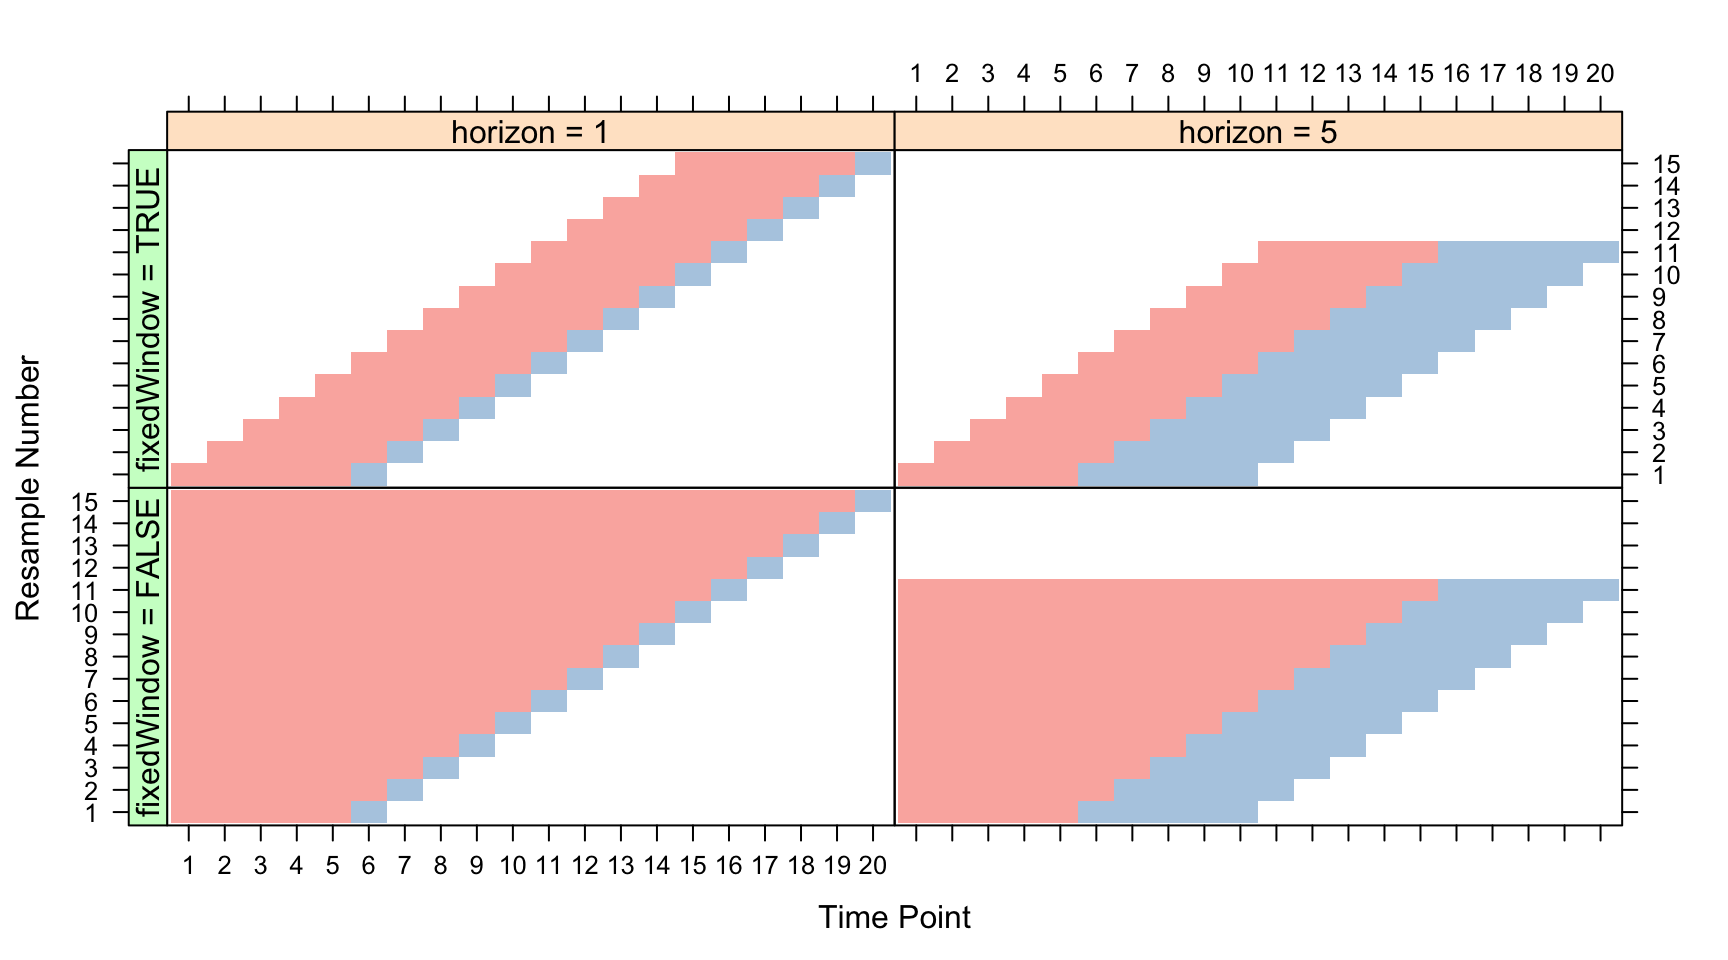
\includegraphics[scale = .23]{windowing_pic_caret}
  \centering
\end{figure}
%% Note: If there is markup in \(sub)section, then it has to be escape as above.
\newpage

A windowing resampling process is created in the function \code{makeResampleDesc()} by supplying the resampling type, horizon, initial window, the length of the series, and an optional argument to skip over some windows for the sake of time.

\begin{knitrout}
\definecolor{shadecolor}{rgb}{0.969, 0.969, 0.969}\color{fgcolor}\begin{kframe}
\begin{alltt}
\hlstd{resampDesc} \hlkwb{=} \hlkwd{makeResampleDesc}\hlstd{(}\hlstr{"GrowingCV"}\hlstd{,} \hlkwc{horizon} \hlstd{=} \hlnum{35L}\hlstd{,}
                               \hlkwc{initial.window} \hlstd{=} \hlnum{.7}\hlstd{,}
                               \hlkwc{size} \hlstd{=} \hlkwd{nrow}\hlstd{(}\hlkwd{getTaskData}\hlstd{(climate.task)),}
                               \hlkwc{skip} \hlstd{=} \hlnum{.02}\hlstd{)}
\hlstd{resampDesc}
\end{alltt}
\begin{verbatim}
## Window description:
##  growing with 14 iterations:
##  448 observations in initial window and 35 horizon.
## Predict: test
## Stratification: FALSE
\end{verbatim}
\end{kframe}
\end{knitrout}


To make a parameter set to tune over \pkg{mlr} uses \pkg{ParamHelpers} ~\cite{paramhelper}. There are several types of tools to help us search our parameter space including grid search, random search ~\cite{Bergstra}, to search our parameter space for the most optimal model.


                                      
\begin{knitrout}
\definecolor{shadecolor}{rgb}{0.969, 0.969, 0.969}\color{fgcolor}\begin{kframe}
\begin{alltt}
\hlstd{parSet} \hlkwb{=} \hlkwd{makeParamSet}\hlstd{(}\hlkwd{makeLogicalParam}\hlstd{(}\hlkwc{id} \hlstd{=} \hlstr{"use.box.cox"}\hlstd{,} \hlkwc{default} \hlstd{=} \hlnum{FALSE}\hlstd{,}
                                     \hlkwc{tunable} \hlstd{=} \hlnum{TRUE}\hlstd{),}
                     \hlkwd{makeLogicalParam}\hlstd{(}\hlkwc{id} \hlstd{=} \hlstr{"use.trend"}\hlstd{,} \hlkwc{default} \hlstd{=} \hlnum{FALSE}\hlstd{,}
                                      \hlkwc{tunable} \hlstd{=} \hlnum{TRUE}\hlstd{),}
                     \hlkwd{makeLogicalParam}\hlstd{(}\hlkwc{id} \hlstd{=} \hlstr{"use.damped.trend"}\hlstd{,}
                                      \hlkwc{default} \hlstd{=} \hlnum{FALSE}\hlstd{,}
                                      \hlkwc{tunable} \hlstd{=} \hlnum{TRUE}\hlstd{),}
                     \hlkwd{makeLogicalParam}\hlstd{(}\hlkwc{id} \hlstd{=} \hlstr{"seasonal.periods"}\hlstd{,}
                                      \hlkwc{default} \hlstd{=} \hlnum{FALSE}\hlstd{,}
                                      \hlkwc{tunable} \hlstd{=} \hlnum{TRUE}\hlstd{),}
                     \hlkwd{makeIntegerParam}\hlstd{(}\hlkwc{id} \hlstd{=} \hlstr{"max.p"}\hlstd{,} \hlkwc{upper} \hlstd{=} \hlnum{10}\hlstd{,} \hlkwc{lower} \hlstd{=} \hlnum{0}\hlstd{),}
                     \hlkwd{makeIntegerParam}\hlstd{(}\hlkwc{id} \hlstd{=} \hlstr{"start.p"}\hlstd{,} \hlkwc{upper} \hlstd{=} \hlnum{10}\hlstd{,} \hlkwc{lower} \hlstd{=} \hlnum{1}\hlstd{,}
                                      \hlkwc{trafo} \hlstd{=} \hlkwa{function}\hlstd{(}\hlkwc{x}\hlstd{) x}\hlopt{*}\hlnum{2}\hlstd{),}
                     \hlkwd{makeIntegerParam}\hlstd{(}\hlkwc{id} \hlstd{=} \hlstr{"max.q"}\hlstd{,} \hlkwc{upper} \hlstd{=} \hlnum{20}\hlstd{,} \hlkwc{lower} \hlstd{=} \hlnum{10}\hlstd{),}
                     \hlkwd{makeIntegerParam}\hlstd{(}\hlkwc{id} \hlstd{=} \hlstr{"start.q"}\hlstd{,} \hlkwc{upper} \hlstd{=} \hlnum{5}\hlstd{,} \hlkwc{lower} \hlstd{=} \hlnum{0}\hlstd{,}
                                      \hlkwc{trafo} \hlstd{=} \hlkwa{function}\hlstd{(}\hlkwc{x}\hlstd{) x}\hlopt{*}\hlnum{2}\hlstd{),}
                     \hlkwd{makeIntegerParam}\hlstd{(}\hlstr{"max.P"}\hlstd{,} \hlkwc{lower} \hlstd{=} \hlnum{0}\hlstd{,} \hlkwc{upper} \hlstd{=} \hlnum{3}\hlstd{),}
                     \hlkwd{makeIntegerParam}\hlstd{(}\hlstr{"max.Q"}\hlstd{,} \hlkwc{lower} \hlstd{=} \hlnum{0}\hlstd{,} \hlkwc{upper} \hlstd{=} \hlnum{2}\hlstd{),}
                     \hlkwd{makeDiscreteParam}\hlstd{(}\hlstr{"ic"}\hlstd{,}
                                       \hlkwc{values} \hlstd{=} \hlkwd{c}\hlstd{(}\hlstr{"aicc"}\hlstd{,}\hlstr{"aic"}\hlstd{,}\hlstr{"bic"}\hlstd{)),}
                     \hlkwd{makeDiscreteParam}\hlstd{(}\hlstr{"test"}\hlstd{,}
                                       \hlkwc{values} \hlstd{=} \hlkwd{c}\hlstd{(}\hlstr{"kpss"}\hlstd{,}\hlstr{"adf"}\hlstd{,}\hlstr{"pp"}\hlstd{)),}
                     \hlkwd{makeDiscreteParam}\hlstd{(}\hlstr{"seasonal.test"}\hlstd{,}
                                       \hlkwc{values} \hlstd{=} \hlkwd{c}\hlstd{(}\hlstr{"ocsb"}\hlstd{,} \hlstr{"ch"}\hlstd{)),}
                     \hlkwd{makeLogicalParam}\hlstd{(}\hlstr{"biasadj"}\hlstd{,} \hlkwc{default} \hlstd{=} \hlnum{FALSE}\hlstd{)}
                     \hlstd{)}

\hlcom{#Specify tune by grid estimation}
\hlstd{ctrl} \hlkwb{=} \hlkwd{makeTuneControlIrace}\hlstd{(}\hlkwc{maxExperiments} \hlstd{=} \hlnum{500L}\hlstd{)}
\end{alltt}
\end{kframe}
\end{knitrout}

Using \code{tuneParams()} the model is tuned for the task using the specified resampling scheme, parameter set, tune control, and measure. For this tuning task we use MASE ~\cite{Hyndman2006} as a measure of performance \footnote{Models with a seasonal difference $> 0$ may be favorably biased as we use the non-seasonal MASE score}.

\begin{knitrout}
\definecolor{shadecolor}{rgb}{0.969, 0.969, 0.969}\color{fgcolor}\begin{kframe}
\begin{alltt}
\hlcom{#}
\hlkwd{library}\hlstd{(}\hlstr{"parallelMap"}\hlstd{)}
\hlkwd{parallelStartSocket}\hlstd{(}\hlnum{6}\hlstd{)}
\hlkwd{configureMlr}\hlstd{(}\hlkwc{on.learner.error} \hlstd{=} \hlstr{"warn"}\hlstd{)}
\hlkwd{set.seed}\hlstd{(}\hlnum{1234}\hlstd{)}
\hlstd{tbatsTune} \hlkwb{=} \hlkwd{tuneParams}\hlstd{(}\hlkwd{makeLearner}\hlstd{(}\hlstr{"fcregr.tbats"}\hlstd{,} \hlkwc{h} \hlstd{=} \hlnum{35}\hlstd{),}
                       \hlkwc{task} \hlstd{= climate.task,} \hlkwc{resampling} \hlstd{= resampDesc,}
                       \hlkwc{par.set} \hlstd{= parSet,} \hlkwc{control} \hlstd{= ctrl,} \hlkwc{measures} \hlstd{= mase)}
\hlkwd{parallelStop}\hlstd{()}
\hlstd{tbatsTune}
\end{alltt}
\end{kframe}
\end{knitrout}

\begin{knitrout}
\definecolor{shadecolor}{rgb}{0.969, 0.969, 0.969}\color{fgcolor}\begin{kframe}
\begin{verbatim}
## Tune result:
## Op. pars: use.box.cox=TRUE; use.trend=TRUE; use.damped.trend=TRUE; seasonal.periods=FALSE; max.p=7; start.p=8; max.q=2; start.q=8; max.P=2; max.Q=1; ic=aicc; test=kpss; seasonal.test=ocsb; biasadj=FALSE; h=35
## mase.test.mean=0.0688
\end{verbatim}
\end{kframe}
\end{knitrout}


The best model's parameters are extracted using \code{setHyperPars()} and the best model is passed to \code{train()} to go over the full data set.

\begin{knitrout}
\definecolor{shadecolor}{rgb}{0.969, 0.969, 0.969}\color{fgcolor}\begin{kframe}
\begin{alltt}
\hlstd{lrn} \hlkwb{=} \hlkwd{setHyperPars}\hlstd{(}\hlkwd{makeLearner}\hlstd{(}\hlstr{"fcregr.tbats"}\hlstd{,} \hlkwc{h} \hlstd{=} \hlnum{35}\hlstd{),}
                   \hlkwc{par.vals} \hlstd{= tbatsTune}\hlopt{$}\hlstd{x)}
\hlstd{m} \hlkwb{=} \hlkwd{train}\hlstd{(lrn, climate.task)}
\end{alltt}
\end{kframe}
\end{knitrout}

To make predictions for our test set we simply pass our model, task, and test data to \code{predict()}

\begin{knitrout}
\definecolor{shadecolor}{rgb}{0.969, 0.969, 0.969}\color{fgcolor}\begin{kframe}
\begin{alltt}
\hlstd{climate.pred} \hlkwb{=} \hlkwd{predict}\hlstd{(m,} \hlkwc{newdata} \hlstd{= m4.test)}
\hlkwd{performance}\hlstd{(climate.pred,} \hlkwc{measures} \hlstd{= mase,} \hlkwc{task} \hlstd{= climate.task)}
\end{alltt}
\begin{verbatim}
##       mase 
## 0.06145902
\end{verbatim}
\end{kframe}
\end{knitrout}

\begin{knitrout}
\definecolor{shadecolor}{rgb}{0.969, 0.969, 0.969}\color{fgcolor}
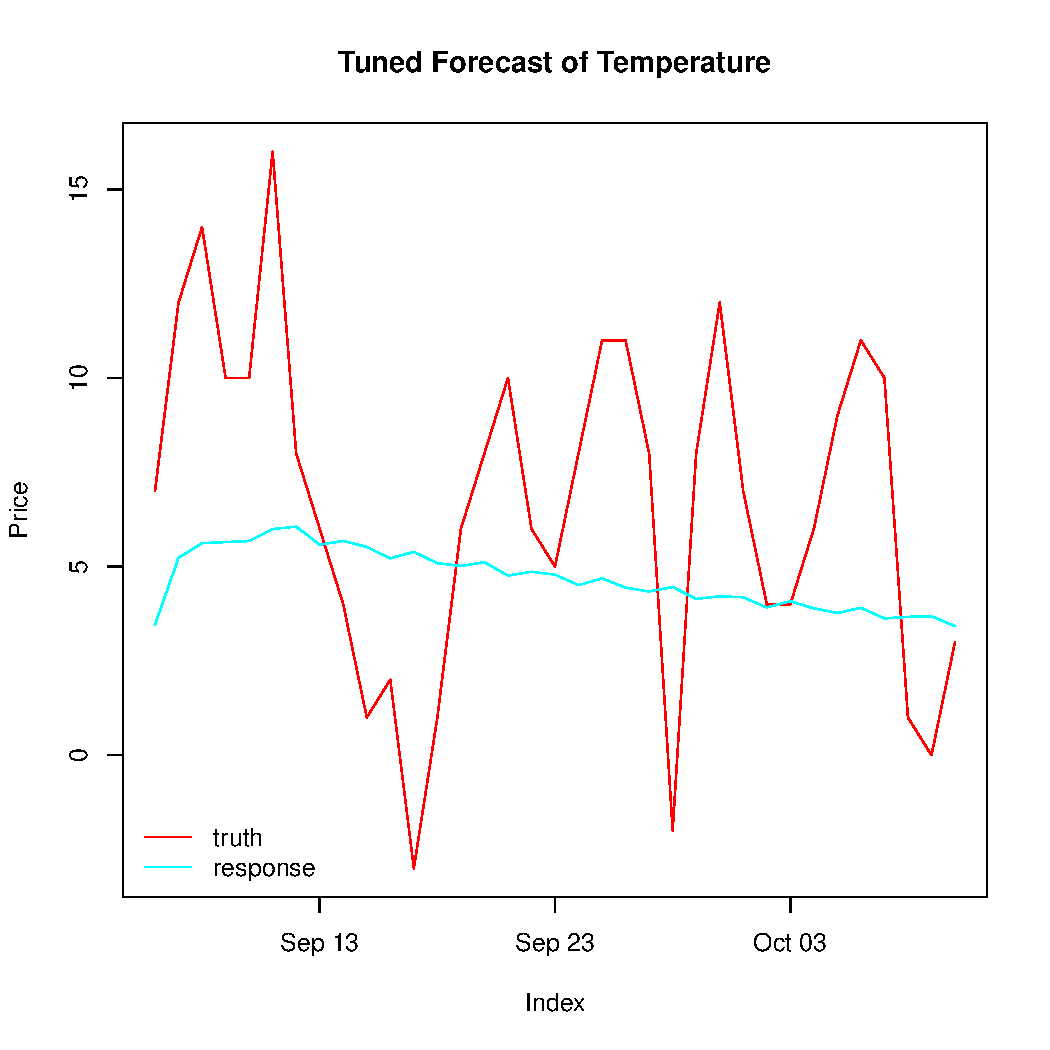
\includegraphics[width=\maxwidth]{figure/plottbatsTune-1} 

\end{knitrout}


\begin{knitrout}
\definecolor{shadecolor}{rgb}{0.969, 0.969, 0.969}\color{fgcolor}\begin{kframe}
\begin{alltt}
\hlstd{par_set} \hlkwb{=} \hlkwd{makeParamSet}\hlstd{(}
  \hlkwd{makeDiscreteParam}\hlstd{(}\hlkwc{id} \hlstd{=} \hlstr{"model"}\hlstd{,} \hlkwc{values} \hlstd{=} \hlkwd{c}\hlstd{(}\hlstr{"sGARCH"}\hlstd{,} \hlstr{"csGARCH"}\hlstd{)),}
  \hlkwd{makeIntegerVectorParam}\hlstd{(}\hlkwc{id} \hlstd{=} \hlstr{"garchOrder"}\hlstd{,} \hlkwc{len} \hlstd{=} \hlnum{2L}\hlstd{,} \hlkwc{lower} \hlstd{=} \hlkwd{c}\hlstd{(}\hlnum{1}\hlstd{,}\hlnum{1}\hlstd{),}
                         \hlkwc{upper} \hlstd{=} \hlkwd{c}\hlstd{(}\hlnum{4}\hlstd{,}\hlnum{4}\hlstd{)),}
  \hlkwd{makeIntegerVectorParam}\hlstd{(}\hlkwc{id} \hlstd{=} \hlstr{"armaOrder"}\hlstd{,} \hlkwc{len} \hlstd{=} \hlnum{2L}\hlstd{,} \hlkwc{lower} \hlstd{=} \hlkwd{c}\hlstd{(}\hlnum{5}\hlstd{,}\hlnum{1}\hlstd{),}
                         \hlkwc{upper} \hlstd{=} \hlkwd{c}\hlstd{(}\hlnum{8}\hlstd{,}\hlnum{3}\hlstd{)),}
  \hlkwd{makeLogicalParam}\hlstd{(}\hlkwc{id} \hlstd{=} \hlstr{"include.mean"}\hlstd{),}
  \hlkwd{makeLogicalParam}\hlstd{(}\hlkwc{id} \hlstd{=} \hlstr{"archm"}\hlstd{),}
  \hlkwd{makeDiscreteParam}\hlstd{(}\hlkwc{id} \hlstd{=} \hlstr{"distribution.model"}\hlstd{,}
                    \hlkwc{values} \hlstd{=} \hlkwd{c}\hlstd{(}\hlstr{"norm"}\hlstd{,}\hlstr{"std"}\hlstd{,}\hlstr{"jsu"}\hlstd{)),}
  \hlkwd{makeDiscreteParam}\hlstd{(}\hlkwc{id} \hlstd{=} \hlstr{"stationarity"}\hlstd{,} \hlkwd{c}\hlstd{(}\hlnum{0}\hlstd{,}\hlnum{1}\hlstd{)),}
  \hlkwd{makeDiscreteParam}\hlstd{(}\hlkwc{id} \hlstd{=} \hlstr{"fixed.se"}\hlstd{,} \hlkwd{c}\hlstd{(}\hlnum{0}\hlstd{,}\hlnum{1}\hlstd{)),}
  \hlkwd{makeDiscreteParam}\hlstd{(}\hlkwc{id} \hlstd{=} \hlstr{"solver"}\hlstd{,} \hlkwc{values} \hlstd{=} \hlstr{"nloptr"}\hlstd{),}
  \hlkwd{makeIntegerParam}\hlstd{(}\hlkwc{id} \hlstd{=} \hlstr{"n.ahead"}\hlstd{,} \hlkwc{default} \hlstd{=} \hlnum{35L}\hlstd{,} \hlkwc{lower} \hlstd{=} \hlnum{35L}\hlstd{,}
                   \hlkwc{upper} \hlstd{=} \hlnum{36L}\hlstd{,} \hlkwc{tunable} \hlstd{=} \hlnum{FALSE}\hlstd{)}
\hlstd{)}

\hlcom{#Specify tune by grid estimation}
\hlstd{ctrl} \hlkwb{=} \hlkwd{makeTuneControlIrace}\hlstd{(}\hlkwc{maxExperiments} \hlstd{=} \hlnum{400L}\hlstd{)}

\hlkwd{parallelStartSocket}\hlstd{(}\hlnum{6}\hlstd{)}
\hlkwd{configureMlr}\hlstd{(}\hlkwc{on.learner.error} \hlstd{=} \hlstr{"warn"}\hlstd{)}
\hlkwd{set.seed}\hlstd{(}\hlnum{1234}\hlstd{)}
\hlstd{garchTune} \hlkwb{=} \hlkwd{tuneParams}\hlstd{(}\hlstr{"fcregr.garch"}\hlstd{,} \hlkwc{task} \hlstd{= climate.task,}
                       \hlkwc{resampling} \hlstd{= resampDesc,} \hlkwc{par.set} \hlstd{= par_set,}
                       \hlkwc{control} \hlstd{= ctrl,} \hlkwc{measures} \hlstd{= mase)}
\hlkwd{parallelStop}\hlstd{()}
\hlstd{garchTune}
\end{alltt}
\end{kframe}
\end{knitrout}

\begin{knitrout}
\definecolor{shadecolor}{rgb}{0.969, 0.969, 0.969}\color{fgcolor}\begin{kframe}
\begin{verbatim}
## Tune result:
## Op. pars: model=sGARCH; garchOrder=4,1; armaOrder=7,2; include.mean=TRUE; archm=FALSE; distribution.model=norm; stationarity=1; fixed.se=0; solver=nloptr; n.ahead=36
## mase.test.mean=0.0789
\end{verbatim}
\end{kframe}
\end{knitrout}

\begin{knitrout}
\definecolor{shadecolor}{rgb}{0.969, 0.969, 0.969}\color{fgcolor}\begin{kframe}
\begin{verbatim}
##       mase 
## 0.05589035
\end{verbatim}
\end{kframe}
\end{knitrout}

\begin{knitrout}
\definecolor{shadecolor}{rgb}{0.969, 0.969, 0.969}\color{fgcolor}
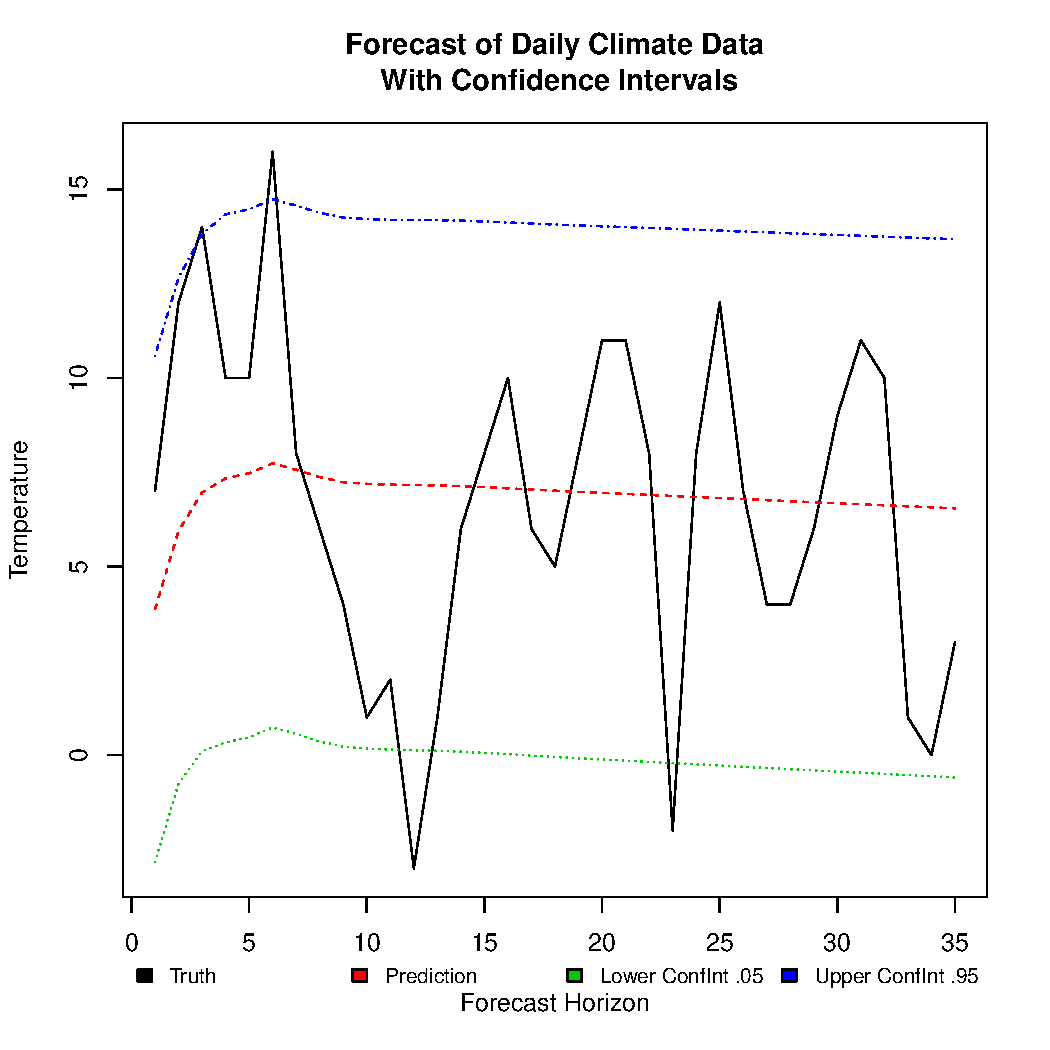
\includegraphics[width=\maxwidth]{figure/garchPlot-1} 

\end{knitrout}

\section{Forecasting with Machine Learning Models}

\subsection{Forecasting with Regression Tasks}

The forecasting extension of \pkg{mlr} includes a preprocessing function that allows supervised machine learning models.

\begin{knitrout}
\definecolor{shadecolor}{rgb}{0.969, 0.969, 0.969}\color{fgcolor}\begin{kframe}
\begin{alltt}
\hlstd{climate.regr.task} \hlkwb{=} \hlkwd{makeRegrTask}\hlstd{(}\hlkwc{id} \hlstd{=} \hlstr{"lagged gbm"}\hlstd{,}
                                 \hlkwc{data} \hlstd{=} \hlkwd{as.data.frame}\hlstd{(m4.train),}
                                 \hlkwc{target} \hlstd{=} \hlstr{"target_var"}\hlstd{)}
\hlstd{climate.task.lag} \hlkwb{=} \hlkwd{createLagDiffFeatures}\hlstd{(climate.regr.task,}
                                         \hlkwc{lag} \hlstd{=} \hlnum{1L}\hlopt{:}\hlnum{100L}\hlstd{,} \hlkwc{difference} \hlstd{=} \hlnum{1L}\hlstd{,}
                                         \hlkwc{seasonal.lag} \hlstd{=} \hlnum{1L}\hlopt{:}\hlnum{2L}\hlstd{,} \hlkwc{na.pad}\hlstd{=}\hlnum{FALSE}\hlstd{)}
\hlstd{climate.task.lag}
\end{alltt}
\begin{verbatim}
## Supervised task: lagged gbm
## Type: regr
## Target: target_var
## Observations: 539
## Features:
## numerics  factors  ordered 
##      100        0        0 
## Missings: FALSE
## Has weights: FALSE
## Has blocking: FALSE
\end{verbatim}
\end{kframe}
\end{knitrout}

Notice that \code{createLagDiffFeatures()} returns a new task with the lagged variables as the new features. Once the lagged task is created the model is trained or tuned like any other.

\begin{knitrout}
\definecolor{shadecolor}{rgb}{0.969, 0.969, 0.969}\color{fgcolor}\begin{kframe}
\begin{alltt}
\hlstd{lag.gbm} \hlkwb{=} \hlkwd{makeLearner}\hlstd{(}\hlstr{"regr.gbm"}\hlstd{,} \hlkwc{par.vals} \hlstd{=} \hlkwd{list}\hlstd{(}\hlkwc{n.trees} \hlstd{=} \hlnum{100}\hlstd{))}
\hlstd{gbm.train} \hlkwb{=} \hlkwd{train}\hlstd{(lag.gbm, climate.task.lag)}
\end{alltt}
\end{kframe}
\end{knitrout}

The \code{forecast()} function allows machine learning models to do arbitary n-step ahead forecasts\footnote{Maybe explain what that means?}.

\begin{knitrout}
\definecolor{shadecolor}{rgb}{0.969, 0.969, 0.969}\color{fgcolor}\begin{kframe}
\begin{alltt}
\hlstd{m4.test.df} \hlkwb{=} \hlkwd{as.data.frame}\hlstd{(m4.test,}\hlkwc{row.names} \hlstd{=} \hlkwd{index}\hlstd{(m4.test))}
\hlstd{gbm.forecast} \hlkwb{=} \hlkwd{forecast}\hlstd{(gbm.train,} \hlkwc{h} \hlstd{=} \hlnum{35L}\hlstd{,}
                        \hlkwc{newdata} \hlstd{= m4.test.df)}
\hlkwd{performance}\hlstd{(gbm.forecast,mase,climate.regr.task)}
\end{alltt}
\begin{verbatim}
##      mase 
## 0.0571994
\end{verbatim}
\end{kframe}
\end{knitrout}

\begin{knitrout}
\definecolor{shadecolor}{rgb}{0.969, 0.969, 0.969}\color{fgcolor}
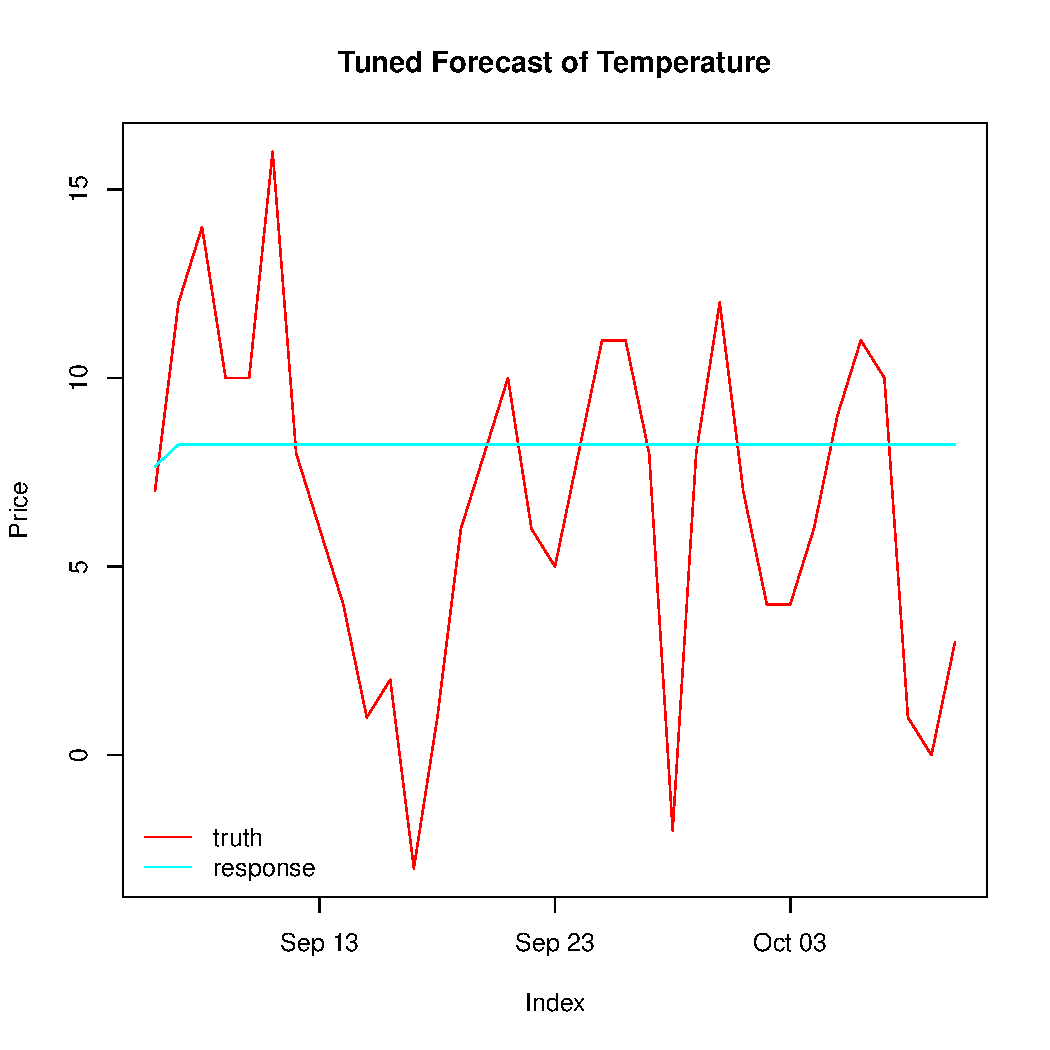
\includegraphics[width=\maxwidth]{figure/forecastgbmplot-1} 

\end{knitrout}

\subsection{Forecasting with Classification Tasks}

For developing trading strategies, we normally have a discrete set of choices such as to buy, sell, or hold onto a stock. Using forecasting in mlr we can now train classification models that forecast these choices. To example this, a simple buy, sell, or hold trading strategy will be built Using the \code{EuStockMarkets}'s DAX index. If the stock goes up by 5\% in a day we will buy, down 5\% we will sell, and otherwise we will hold onto the current stocks we have. 

\begin{knitrout}
\definecolor{shadecolor}{rgb}{0.969, 0.969, 0.969}\color{fgcolor}\begin{kframe}
\begin{alltt}
\hlstd{DAX} \hlkwb{=} \hlstd{EuStockMarkets}\hlopt{$}\hlstd{DAX}\hlopt{/}\hlkwd{lag}\hlstd{(EuStockMarkets}\hlopt{$}\hlstd{DAX,}
                             \hlnum{7}\hlstd{,}\hlkwc{nap.pad} \hlstd{=} \hlnum{FALSE}\hlstd{)} \hlopt{-} \hlnum{1}
\hlstd{trade.strat} \hlkwb{=} \hlkwd{ifelse}\hlstd{(DAX} \hlopt{>} \hlnum{.02}\hlstd{,} \hlstr{"Buy"}\hlstd{,}
                     \hlkwd{ifelse}\hlstd{(DAX} \hlopt{< -}\hlnum{.01}\hlstd{,} \hlstr{"Sell"}\hlstd{,} \hlstr{"Hold"}\hlstd{))}
\hlstd{trade.strat} \hlkwb{=} \hlstd{trade.strat[}\hlnum{8}\hlopt{:}\hlnum{1860}\hlstd{]}
\hlstd{euro.classif.data} \hlkwb{=} \hlkwd{data.frame}\hlstd{(}\hlkwc{trade.strat} \hlstd{= trade.strat ,}
                               \hlkwc{row.names} \hlstd{=} \hlkwd{index}\hlstd{(trade.strat))}

\hlstd{euro.classif.train} \hlkwb{=} \hlstd{euro.classif.data[}\hlnum{1}\hlopt{:}\hlnum{1821}\hlstd{,,}\hlkwc{drop} \hlstd{=} \hlnum{FALSE}\hlstd{]}
\hlstd{euro.classif.test}  \hlkwb{=} \hlstd{euro.classif.data[}\hlnum{1822}\hlopt{:}\hlnum{1853}\hlstd{,,}\hlkwc{drop} \hlstd{=} \hlnum{FALSE}\hlstd{]}
\hlstd{classif.task} \hlkwb{=} \hlkwd{makeClassifTask}\hlstd{(}\hlkwc{data} \hlstd{= euro.classif.train,}
                               \hlkwc{target} \hlstd{=} \hlstr{"DAX"}\hlstd{)}
\hlstd{classif.task.lag} \hlkwb{=} \hlkwd{createLagDiffFeatures}\hlstd{(classif.task,}
                                         \hlkwc{lag} \hlstd{=} \hlnum{1L}\hlopt{:}\hlnum{365L}\hlstd{,}
                                         \hlkwc{na.pad} \hlstd{=} \hlnum{FALSE}\hlstd{)}
\hlstd{classif.learn} \hlkwb{=} \hlkwd{makeLearner}\hlstd{(}\hlstr{"classif.boosting"}\hlstd{,} \hlkwc{xval} \hlstd{=} \hlnum{1}\hlstd{,}
                            \hlkwc{mfinal} \hlstd{=} \hlnum{200}\hlstd{,} \hlkwc{minsplit} \hlstd{=} \hlnum{10}\hlstd{)}
\end{alltt}
\end{kframe}
\end{knitrout}

\begin{knitrout}
\definecolor{shadecolor}{rgb}{0.969, 0.969, 0.969}\color{fgcolor}\begin{kframe}
\begin{alltt}
\hlstd{classif.train} \hlkwb{=} \hlkwd{train}\hlstd{(classif.learn, classif.task.lag)}
\hlstd{classif.fc} \hlkwb{=} \hlkwd{forecast}\hlstd{(classif.train,} \hlkwc{h}\hlstd{=}\hlnum{32}\hlstd{,} \hlkwc{newdata} \hlstd{= euro.classif.test)}
\hlkwd{performance}\hlstd{(classif.fc)}
\end{alltt}
\end{kframe}
\end{knitrout}

\begin{knitrout}
\definecolor{shadecolor}{rgb}{0.969, 0.969, 0.969}\color{fgcolor}\begin{kframe}
\begin{verbatim}
## Prediction: 32 observations
## predict.type: response
## threshold: 
## time: 125.91
##   truth response
## 1   Buy      Buy
## 2   Buy      Buy
## 3  Hold      Buy
## 4  Hold      Buy
## 5  Hold      Buy
## 6   Buy      Buy
## ... (32 rows, 2 cols)
##   mmce 
## 0.6875
\end{verbatim}
\end{kframe}
\end{knitrout}

\section{Lambert W Transforms}

Many machine learning and time series models rely one the assumption that our data or errors fit a normal distribution. This assumption becomes precarious when modeling the asymmetric and fat-tailed data of the real world. Lambert W Transforms are a family of generalized skewed distributions ~\cite{LambertGeneral} that have bijecetive and parametric functions that allow heavy tailed and asymettric data to appear more Gaussian  ~\cite{GaussLam}. 

Let $U$ be a continuous random variable with cdf $F_U(u|\beta)$ and pdf $f_U(u|\beta)$ given $\beta$ is a parameter vector. Define a continuous location-scale random variable $X\sim F_X(x|\beta)$. A locaton-scale skewed Lambert $W\times F_X$ random variable is defined as 
\begin{equation}
Z = U\exp\left(\frac{\delta}{2}(U^2)^\right),\; \delta\ge 0
\end{equation}
And the heavy-tailed Lambert $W\times F_X$ random variable can be defined as
\begin{equation}
Z = U\exp\left(\frac{\delta}{2}(U^2)^\alpha\right),\; \delta\ge 0\; \alpha > 0
\end{equation}

Given that $U = (X-\mu_X)/\sigma_X$ where $\mu_X$, $\sigma_X$, $\delta$, and $\alpha$ are the mean and standard deviation of X and the parameters to control skewness and asymetry , respectively. When $\delta = 0$, equation 12 reduces to a standard normal distribution. Equation 12 is the general form of Tukey's $h$ distribution ~\cite{ghdist} and the basis for Morgenthaler and Tukey's ~\cite{hhdist} skewed, heavy tailed family of $hh$ random variables.

\begin{equation}
  Z = \begin{cases}
               U\exp\left(\frac{\delta_l}{2}(U^2)^\alpha_l\right),\; \delta_l \ge 0\; \alpha_l > 0\\
               U\exp\left(\frac{\delta_r}{2}(U^2)^\alpha_r\right),\; \delta_r \ge 0 \alpha_r > 0
            \end{cases}
\end{equation}

\begin{knitrout}
\definecolor{shadecolor}{rgb}{0.969, 0.969, 0.969}\color{fgcolor}
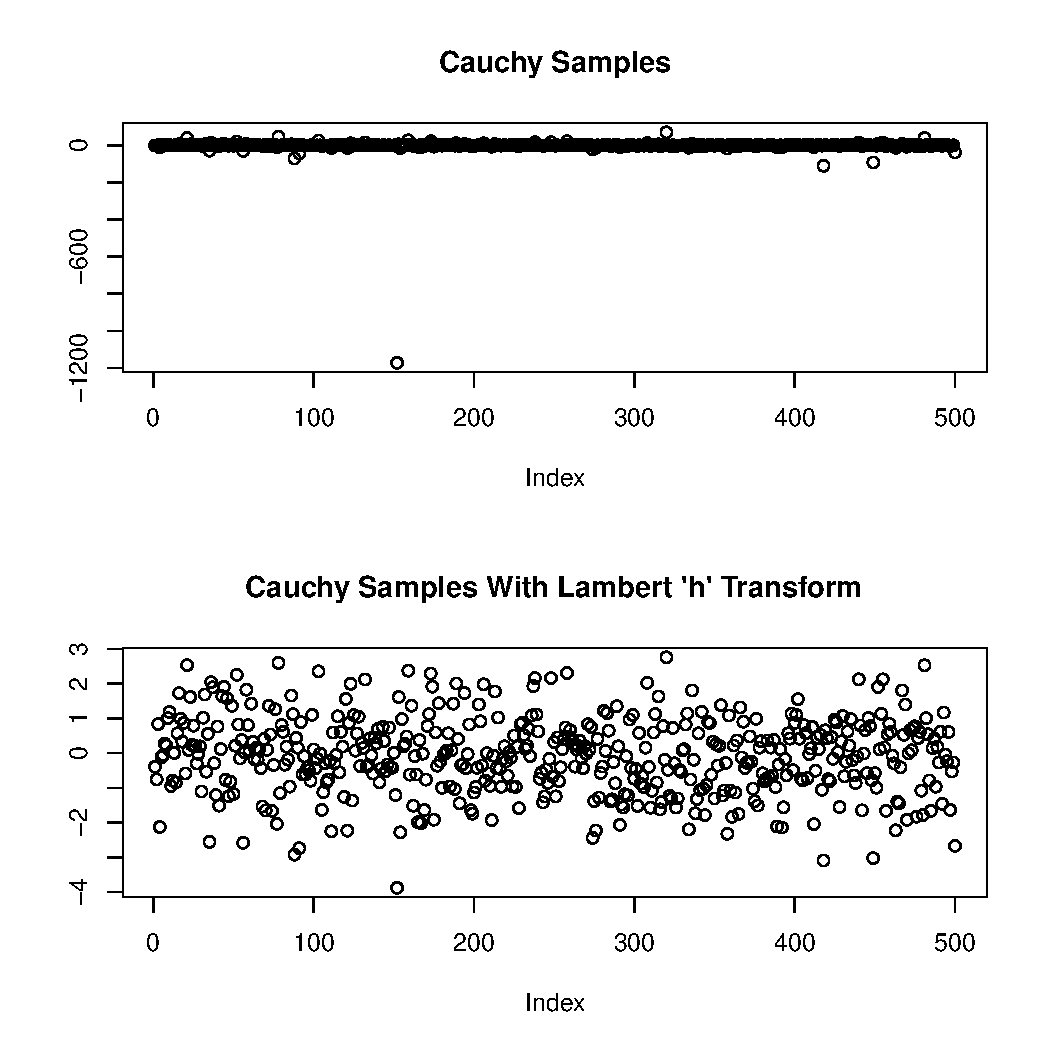
\includegraphics[width=\maxwidth]{figure/lambertWplots-1} 

\end{knitrout}

The function \code{Gaussianize} is available in the package \pkg{LambertW} and has been made into a preprocessing function in \pkg{mlr}.

\begin{knitrout}
\definecolor{shadecolor}{rgb}{0.969, 0.969, 0.969}\color{fgcolor}\begin{kframe}
\begin{alltt}
\hlcom{# Need to make this more dramatic}
\hlstd{lamb.lrn} \hlkwb{=} \hlkwd{makePreprocWrapperLambert}\hlstd{(}\hlstr{"classif.lda"}\hlstd{,} \hlkwc{type} \hlstd{=} \hlstr{"h"}\hlstd{)}
\hlstd{lamb.lrn}
\end{alltt}
\begin{verbatim}
## Learner classif.lda.preproc from package MASS
## Type: classif
## Name: ; Short name: 
## Class: PreprocWrapperLambert
## Properties: numerics,factors,prob,twoclass,multiclass
## Predict-Type: response
## Hyperparameters: type=h,methods=IGMM,verbose=FALSE
\end{verbatim}
\begin{alltt}
\hlstd{lamb.trn} \hlkwb{=} \hlkwd{train}\hlstd{(lamb.lrn,iris.task,} \hlkwc{subset} \hlstd{=} \hlnum{1}\hlopt{:}\hlnum{120}\hlstd{)}
\hlstd{lamb.pred} \hlkwb{=} \hlkwd{predict}\hlstd{(lamb.trn, iris.task,} \hlkwc{subset} \hlstd{=} \hlnum{121}\hlopt{:}\hlnum{150}\hlstd{)}

\hlcom{# Do the non-LW version}
\hlstd{trn} \hlkwb{=} \hlkwd{train}\hlstd{(}\hlkwd{makeLearner}\hlstd{(}\hlstr{"classif.lda"}\hlstd{),iris.task,} \hlkwc{subset} \hlstd{=} \hlnum{1}\hlopt{:}\hlnum{120}\hlstd{)}
\hlstd{pred} \hlkwb{=} \hlkwd{predict}\hlstd{(trn, iris.task,} \hlkwc{subset} \hlstd{=} \hlnum{121}\hlopt{:}\hlnum{150}\hlstd{)}
\hlkwd{performance}\hlstd{(lamb.pred)}
\end{alltt}
\begin{verbatim}
## mmce 
##  0.1
\end{verbatim}
\begin{alltt}
\hlkwd{performance}\hlstd{(pred)}
\end{alltt}
\begin{verbatim}
## mmce 
##  0.1
\end{verbatim}
\end{kframe}
\end{knitrout}


\section{Ensembles of Forecasting Models}

\begin{knitrout}
\definecolor{shadecolor}{rgb}{0.969, 0.969, 0.969}\color{fgcolor}\begin{kframe}
\begin{alltt}
\hlstd{resamp.sub} \hlkwb{=} \hlkwd{makeResampleDesc}\hlstd{(}\hlstr{"GrowingCV"}\hlstd{,}
                          \hlkwc{horizon} \hlstd{=} \hlnum{35L}\hlstd{,}
                          \hlkwc{initial.window} \hlstd{=} \hlnum{.90}\hlstd{,}
                          \hlkwc{size} \hlstd{=} \hlkwd{nrow}\hlstd{(}\hlkwd{getTaskData}\hlstd{(climate.task)),}
                          \hlkwc{skip} \hlstd{=} \hlnum{.01}
                          \hlstd{)}

\hlstd{lrns} \hlkwb{=} \hlkwd{makeLearners}\hlstd{(}\hlkwd{c}\hlstd{(}\hlstr{"fcregr.tbats"}\hlstd{,}\hlstr{"fcregr.garch"}\hlstd{,} \hlstr{"fcregr.arfima"}\hlstd{))}


\hlstd{stack.forecast} \hlkwb{=} \hlkwd{makeStackedLearner}\hlstd{(}\hlkwc{base.learners} \hlstd{= lrns,}
                       \hlkwc{predict.type} \hlstd{=} \hlstr{"response"}\hlstd{,}
                       \hlkwc{method} \hlstd{=} \hlstr{"average"}\hlstd{)}

\hlcom{# Simple param set for tuning sub learners}
\hlstd{ps} \hlkwb{=} \hlkwd{makeParamSet}\hlstd{(}
  \hlkwd{makeDiscreteParam}\hlstd{(}\hlstr{"fcregr.tbats.h"}\hlstd{,} \hlkwc{values} \hlstd{=} \hlnum{32}\hlstd{),}
  \hlkwd{makeDiscreteParam}\hlstd{(}\hlstr{"fcregr.garch.n.ahead"}\hlstd{,} \hlkwc{values} \hlstd{=} \hlnum{32}\hlstd{),}
  \hlkwd{makeDiscreteParam}\hlstd{(}\hlstr{"fcregr.arfima.h"}\hlstd{,} \hlkwc{values} \hlstd{=} \hlnum{32}\hlstd{),}
  \hlkwd{makeDiscreteParam}\hlstd{(}\hlstr{"fcregr.arfima.estim"}\hlstd{,} \hlkwc{values} \hlstd{=} \hlstr{"ls"}\hlstd{),}
  \hlkwd{makeIntegerParam}\hlstd{(}\hlstr{"fcregr.arfima.max.P"}\hlstd{,} \hlkwc{lower} \hlstd{=} \hlnum{0}\hlstd{,} \hlkwc{upper} \hlstd{=} \hlnum{3}\hlstd{),}
  \hlkwd{makeIntegerParam}\hlstd{(}\hlstr{"fcregr.arfima.max.Q"}\hlstd{,} \hlkwc{lower} \hlstd{=} \hlnum{0}\hlstd{,} \hlkwc{upper} \hlstd{=} \hlnum{2}\hlstd{),}
  \hlkwd{makeDiscreteParam}\hlstd{(}\hlstr{"fcregr.arfima.ic"}\hlstd{,} \hlkwc{values} \hlstd{=} \hlkwd{c}\hlstd{(}\hlstr{"aicc"}\hlstd{,}\hlstr{"aic"}\hlstd{,}\hlstr{"bic"}\hlstd{)),}
  \hlkwd{makeDiscreteParam}\hlstd{(}\hlkwc{id} \hlstd{=} \hlstr{"model"}\hlstd{,} \hlkwc{values} \hlstd{=} \hlkwd{c}\hlstd{(}\hlstr{"sGARCH"}\hlstd{,} \hlstr{"csGARCH"}\hlstd{)),}
  \hlkwd{makeIntegerVectorParam}\hlstd{(}\hlkwc{id} \hlstd{=} \hlstr{"fcregr.garch.garchOrder"}\hlstd{,}
                         \hlkwc{len} \hlstd{=} \hlnum{2L}\hlstd{,} \hlkwc{lower} \hlstd{=} \hlkwd{c}\hlstd{(}\hlnum{1}\hlstd{,}\hlnum{1}\hlstd{),}
                         \hlkwc{upper} \hlstd{=} \hlkwd{c}\hlstd{(}\hlnum{4}\hlstd{,}\hlnum{4}\hlstd{)),}
  \hlkwd{makeIntegerVectorParam}\hlstd{(}\hlkwc{id} \hlstd{=} \hlstr{"fcregr.garch.armaOrder"}\hlstd{,}
                         \hlkwc{len} \hlstd{=} \hlnum{2L}\hlstd{,} \hlkwc{lower} \hlstd{=} \hlkwd{c}\hlstd{(}\hlnum{5}\hlstd{,}\hlnum{1}\hlstd{),}
                         \hlkwc{upper} \hlstd{=} \hlkwd{c}\hlstd{(}\hlnum{8}\hlstd{,}\hlnum{3}\hlstd{)),}
  \hlkwd{makeLogicalParam}\hlstd{(}\hlkwc{id} \hlstd{=} \hlstr{"fcregr.garch.archm"}\hlstd{),}
  \hlkwd{makeDiscreteParam}\hlstd{(}\hlkwc{id} \hlstd{=} \hlstr{"fcregr.garch.distribution.model"}\hlstd{,}
                    \hlkwc{values} \hlstd{=} \hlkwd{c}\hlstd{(}\hlstr{"norm"}\hlstd{,}\hlstr{"std"}\hlstd{)),}
  \hlkwd{makeLogicalParam}\hlstd{(}\hlkwc{id} \hlstd{=} \hlstr{"fcregr.tbats.use.box.cox"}\hlstd{,}
                                \hlkwc{default} \hlstd{=} \hlnum{FALSE}\hlstd{,}\hlkwc{tunable} \hlstd{=} \hlnum{TRUE}\hlstd{),}
  \hlkwd{makeIntegerParam}\hlstd{(}\hlstr{"fcregr.tbats.max.P"}\hlstd{,} \hlkwc{lower} \hlstd{=} \hlnum{0}\hlstd{,} \hlkwc{upper} \hlstd{=} \hlnum{3}\hlstd{),}
  \hlkwd{makeIntegerParam}\hlstd{(}\hlstr{"fcregr.tbats.max.Q"}\hlstd{,} \hlkwc{lower} \hlstd{=} \hlnum{0}\hlstd{,} \hlkwc{upper} \hlstd{=} \hlnum{2}\hlstd{),}
  \hlkwd{makeDiscreteParam}\hlstd{(}\hlstr{"fcregr.tbats.ic"}\hlstd{,} \hlkwc{values} \hlstd{=} \hlkwd{c}\hlstd{(}\hlstr{"aicc"}\hlstd{,}\hlstr{"aic"}\hlstd{,}\hlstr{"bic"}\hlstd{)),}
  \hlkwd{makeDiscreteParam}\hlstd{(}\hlstr{"fcregr.tbats.test"}\hlstd{,} \hlkwc{values} \hlstd{=} \hlkwd{c}\hlstd{(}\hlstr{"kpss"}\hlstd{,}\hlstr{"adf"}\hlstd{,}\hlstr{"pp"}\hlstd{))}
\hlstd{)}

\hlcom{## tuning}
\hlkwd{parallelStartSocket}\hlstd{(}\hlnum{6}\hlstd{)}
\hlkwd{configureMlr}\hlstd{(}\hlkwc{on.learner.error} \hlstd{=} \hlstr{"warn"}\hlstd{)}
\hlkwd{set.seed}\hlstd{(}\hlnum{1234}\hlstd{)}
\hlstd{fore.tune} \hlkwb{=} \hlkwd{tuneParams}\hlstd{(stack.forecast, fcregr.task,} \hlkwc{resampling} \hlstd{= resamp.sub,}
                   \hlkwc{par.set} \hlstd{= ps,} \hlkwc{control} \hlstd{=} \hlkwd{makeTuneControlGrid}\hlstd{(),}
                   \hlkwc{measures} \hlstd{= mase,} \hlkwc{show.info} \hlstd{=} \hlnum{FALSE}\hlstd{)}
\hlkwd{parallelStop}\hlstd{()}
\hlstd{fore.tune}

\hlcom{# get hyper params}
\hlstd{stack.forecast.tune}  \hlkwb{=} \hlkwd{setHyperPars2}\hlstd{(stack.forecast,fore.tune}\hlopt{$}\hlstd{x)}
\hlstd{stack.forecast.tune}

\hlcom{# Train the final best models and predict}
\hlstd{stack.forecast.mod} \hlkwb{=} \hlkwd{train}\hlstd{(stack.forecast.tune,fcregr.task)}
\hlstd{stack.forecast.pred} \hlkwb{=} \hlkwd{predict}\hlstd{(stack.forecast.mod,} \hlkwc{newdata} \hlstd{= dat.test)}
\hlstd{stack.forecast.pred}
\end{alltt}
\end{kframe}
\end{knitrout}
\newpage
%\small
\bibliography{thesisbib}{}
\bibliographystyle{plain}

\end{document}
